\documentclass{article}
\usepackage{graphicx}
\usepackage{wrapfig}
\usepackage{subcaption}
\usepackage[margin=1in]{geometry}
\usepackage{amsmath} % or simply amstext
\usepackage{amssymb}
\usepackage{siunitx}
\usepackage{booktabs}
\usepackage[export]{adjustbox}
\newcommand{\angstrom}{\textup{\AA}}
\newcommand{\colormap}{jet}  % colorbar to use
\usepackage{cleveref}
\usepackage{booktabs}
\usepackage{gensymb}
\usepackage{float}

%BJC: potential titles (uncommented is current favorite)
%\title{The Transport Mechanisms of Polar Solutes in a Cross-linked H\textsubscript{II} Phase Lyotropic Liquid Crystal Membrane}
\title{Size, Shape and Functionality Dependence of Solute Transport Mechanisms in a Cross-linked H\textsubscript{II} Phase Lyotropic Liquid Crystal Membrane}
\author{Benjamin J. Coscia \and Michael R. Shirts} 

\begin{document}

  \graphicspath{{./figures/}}
  \maketitle

  \section{Introduction}

  We need highly selective membranes in order to perform efficient separations.

  H\textsubscript{II} phase lyotropic liquid crystals have densely packed, uniform
  sized pores and have the potential to disrupt conventional membrane separation
  techniques by being selective based not only on size and charge, but on chemical
  functionality as well.

  We can only learn so much from experiment. MD can give us mechanistic insights with
  atomistic resolution so that we can intelligently design new membranes for 
  solute-specific separations.

  In previous work, we determined the most likely structure of the hexagonal phase 
  formed by the monomer Na-GA3C11.
  \begin{itemize}
  	\item We developed techniques for equilibrating the hexagonal phase made by
	neat monomer as well as with varying amounts of water in the pores.
  \end{itemize} 

  In this work, we have studied the transport mechanisms exhibited by a number
  of polar solutes with varying size, chemical functionality and hydrophilic character.
  \begin{itemize}
	\item Many of the separations we are interested in involve polar organic 
	compounds.
  \end{itemize} 
  
  There are a number of questions that we wish to answer in order to create a
  framework for studying this system in even greater detail.
  \begin{enumerate}
  
   	\item What transport mechanisms do we observe?
  	
  	Given that the pores will restrict motion of the solutes, we anticipate that 
  	transport will be hindered in some way. We want to understand the differences in
  	solute motion, specifically its mean squared displacement (MSD), based on a solute's
  	size and chemical identity (functional groups). We will study the interactions
  	between solutes, the membrane, and water in order to determine which mechanism
  	or mechanisms dominate.
  	
%  	are dictated by a 
%  	solute's chemical identity and if so, what interactions lead to this
%  	difference.
  
  	\item How do molecules, including water, partition within the pores?
  	
  	From a macroscopic perspective, it is straightforward to hypothesize that the water and
  	polar solutes spend their time exclusively in the tube-like hydrophilic pore region.
  	Our previous work showed that there is a gradual compositional transition from the 
  	hydrophilic to the hydrophobic region which means that solutes may not 
  	necessarily stay confined to the centers of the pores or even within the
  	pore region. We will study the gradient in composition of solutes and water
  	and any resultant influence it might have on mechanistic properties.
  	
  	\item Can we describe the transport mechanisms using pre-existing 
  	mathematical models.
  	
  	A mathematical model may provide additional insight into the transport
  	mechanisms and, in future work, can help relate performance on the 
  	timescales studied with MD to macroscopic timescales. We will use
  	qualitative and semi-quantitative arguments in order to choose a 
  	governing model. 
  	
  	\item How can we modify the current monomers in order to enhance
  	solute-specific separations? 
  	
  	Most experimental characterization up to this point has been centered 
  	around the monomer, Na-GA3C11, studied here. The primary reason for conducting
  	these simulations is to understand what chemical modifications can be made 
  	to this or similar liquid crystal molecules in order to enhance transport 
  	of desired species or restrict that of undesired species. We will use the 
  	insight gained from our mechanistic observations in order to suggest new 
  	monomer designs.
  	
  \end{enumerate} 
  
  There are number of questions this study is not intended to answer.
  \begin{itemize}
    \item We will not study the concentration dependence of the observed
    transport rates. Although the average MSD might change with concentration,
    we are focused on the underlying interactions leading to the observed 
    transport mechanisms which we conjecture will be the same regardless of
    concentration.
    \item We will not study the chemical potential of solutes in the pores, which
    could give us a better understanding of equilibrium solute partitioning.
    However, this information will not greatly enhance our understanding of 
    mechanistic details in various membrane regions.
    \item Both of the above points will add unnecessary levels of complexity
    which can be left for a future study. 
%    \item Our work is meant as a simple starting point for studying transport
%    mechanisms in these complex LLC systems.
    \item This work is a simple starting point meant for observing the types
    of interactions which occur between isolated solutes and the membrane.
  \end{itemize}

  \section{Methods}

  \subsection{Molecular Dynamics Simulations}
  
  \subsubsection*{System Setup}

  Stable H\textsubscript{II} phases, assembled with Na-GA3C11, can be formed
  using a broad range of water concentrations.
  \begin{itemize}
	\item In the literature, this system is typically synthesized with close
	to 10 wt \% water \cite{smith_ordered_1997, zhou_new_2007}
    \item However, Resel et al. noted that the system is likely fully 
	hydrated with less than 7 wt \% water. \cite{resel_h2-phase_2000}
	\item We decided to test two different levels of water content: 5 and 10 wt \%
  \end{itemize} 

  We observed that water partitions into the tail region of our system and therefore
  built our initial configurations with water in both regions close to the expected
  equilibrium value.
  \begin{itemize}
	\item There is about 2:1 water in the pores versus in the tails for the 10 wt \% system.
	\item The amount of water present in the tails may or may not be experimentally consistent
	but if we don't put it in, the results will not be thermodynamically consistent, which 
	will give issues with measurements and calculations.
	\item See supporting info for water equilibration simulation data.
	\item We adjusted the pore radius in our systems so that the right amount of water
	fits in the pores without any vacuum using \texttt{gmx solvate}.
	\item We placed water molecules in the tail region one at a time in random locations
	with short energy minimizations between insertions.
  \end{itemize}

%  We equilibrated the initial configuration using the `wet' equilibration procedure
%  described in our previous work (reference to structure paper).
  %BJC: not sure I need to go into any details describing that procedure
%  \begin{itemize}
%	\item Series of NVT simulations with force constants on carbon atoms of aromatic
%	ring in head group
%	\item Force constants reduced according to the sequence: 1000000, 3162,
%	56, 8, 3, 2, 1, 0 kJ mol$^{-1}$ nm$^{-2}$ 
%  \end{itemize}

%  We cross-linked the equilibrated solvated configuration using the cross-linking procedure
%  described in our previous work. 

  We equilibrated an initial solvated configuration before adding solutes.
  \begin{itemize}
	\item We equilibrated the initial configuration using the `wet'
	equilibration procedure described in our previous work~\cite{coscia_understanding_2019}.
	\item We cross-linked the equilibrated solvated configuration using the
	cross-linking procedure described in our previous work. 
  \end{itemize}

  We added 6 solute molecules to each pore of the equilibrated cross-linked
  configuration.
  \begin{itemize}
	\item We equally spaced each solute in the pore
	\item 6 solutes per pore provided a balance of a useful amount of data
	for generating statistics and a low degree of interaction between solutes (reference
	to supporting information to show low degree of interaction)
	\item At each insertion point we placed a randomly oriented solute molecule
	then ran a short energy minimization.
	\item We allowed the solutes to equilibrate for 5 ns using berendsen 
	pressure control
	\item We collected transport data using 1 $\mu$s simulations
  \end{itemize}
  
%  \subsubsection*{Modeling subdiffusion}\label{method:model_sFBM}
%
%  Solutes in our H\textsubscript{II} LLC membrane exhibit subdiffusive
%  behavior, a type of anomalous diffusion. 
%  \begin{itemize}
%  	\item During an anomalous diffusion process, the mean squared displacement (MSD)
%  	does not grow linearly with time, rather it is of the form:
%	\begin{equation} 
%	\langle x^2(t) \rangle = K_{\alpha}t^\alpha
%	\label{eqn:msd_form}
%	\end{equation} 
%	where $\alpha$ is the anomalous exponent and $K_\alpha$ is the
%	generalized diffusion coefficient.
%	\item A value of $\alpha < 1$ indicates a subdiffusive process, while a value of
%	$\alpha = 1$ and $\alpha > 0$ is characteristic of Brownian and superdiffusive
%	motion respectively.
%  \end{itemize}
%
%  \noindent We calculated both the ensemble-averaged and time-averaged MSDs
%  of the simulated trajectories.
%  \begin{itemize}
%	\item The ensemble-averaged MSD measures the displacement of a particle from its initial
%	position~\cite{meroz_toolbox_2015} and can be written as
%	\begin{equation}
%	\langle x^2(t) \rangle = \langle x(t) - x(0) \rangle
%	\label{eqn:ensemble_msd}
%	\end{equation}
%%	\item The average MSD calculated in this way recovers the form of
%%	Equation~\ref{eqn:msd_form}. % time-averaged should recover it too for FBM 
%	\item The time-averaged MSD measures the displacement between all possible time lags
%	and can be written as
%	\begin{equation}
%	\overline{x^2(\tau)} = \dfrac{1}{T - \tau}\int_{0}^{T - \tau} (x(t + \tau) - x(t))^2 dt
%	\end{equation}
%	where $\tau$ is the time lag and T is the length of the
%	trajectory~\cite{meroz_toolbox_2015}. 
%%	\item The time-averaged MSD becomes linear in our simulations,
%%	therefore we can fit a line to its slope in order to estimate the macroscopic
%%	diffusivity of the particle.
%	%BJC: this needs more justification. Not many people have done it
%	%BJC: could also not report them as diffusivities. Comparison of total MSD
%	% should give same information
%	% Linear region probably exists because dwell times on the order of large lag times
%	% become negligible
%  \end{itemize}
%  
%  \noindent Three common mathematical models for modeling anomalous subdiffusion processes include 
%  continuous time random walks (CTRW), fractional Brownian motion (FBM) and
%  random walks on fractals (RWF).\cite{meroz_toolbox_2015}
%  \begin{itemize}
%    \item FBM is common in crowded, viscoelastic environments where each step comes 
%    from a Gaussian distribution but is anti-correlated to its previous 
%    step.~\cite{mandelbrot_fractional_1968,jeon_fractional_2010,banks_anomalous_2005}
%    \item A CTRW is characterized by a distribution of hop lengths and 
%    dwell times, where each each step is characterized by independent random draws from 
%    each distribution.\cite{montroll_random_1965,morrin_three_2018}
%    \item An RWF is imposed by a system's geometry. Systems with tortuous pathways and dead
%    ends cause anti-correlated motion.\cite{meroz_toolbox_2015,neusius_subdiffusion_2008}
%    \item The processes described above can happen alone or in combination.  	
%  \end{itemize}
%  
%  \noindent We believe that solutes in the system studied here exhibit subordinated 
%  fractional Brownian motion (sFBM) where the parent process is FBM and the 
%  leading process is a CTRW. 
%  \begin{itemize}
%  	\item The ensemble-averaged MSD differs from the time-averaged MSD, which
%  	is indicative of non-ergodicity, a trait inherent to CTRWs but not FBM or RWFs.~\cite{thiel_weak_2014}
%  	\item We also observe non-stationary $z$-coordinate traces of each solute's
%  	center of mass (COM). %BJC: figure of a z-coordinate trace in main text or in supporting info
%  	\item For a pure CTRW, the time-averaged MSD should be linear.
%  	~\cite{neusius_subdiffusion_2008,meroz_subdiffusion_2010}
%  	\item However, a typical time-averaged solute MSD is sublinear (see supporting
%  	information), which suggests that there is another underlying subdiffusive mechanism.
%  	\item The hop lengths recorded after each dwell period are anti-correlated (See supporting information)
%  	\item Given the viscoelastic nature of the monomers in our system, we believe
%  	the hop lengths can be modeled with FBM. 
% 	\item For subordinated FBM, it can be shown that
%  	\begin{equation}
%  	\langle x^2(t) \rangle \simeq t^{\alpha\beta}
%  	\end{equation}
%  	where $\alpha$ is the anomalous exponent characteristic of the leading CTRW process
%  	and $\beta$ is the anomalous exponent characteristic of the parent FBM process. 
%  \end{itemize}
%
%  \noindent We can characterize a CTRW process using the parameters which describe its
%  dwell time and hop length distribution.
%  \begin{itemize}
%	\item We used the \texttt{ruptures} python package in order to identify
%	breakpoints in solute trajectories.\cite{truong_ruptures:_2018} (See Supporting Information for more
%	details on chosen parameters. i.e. type of cost function, cost function penalty
%	tolerance, number of dimensions used)
%	\item The corresponding hop lengths and dwell times between break points were 
%	used to construct empirical distributions.
%	\item For solutes in our system, the distribution of hop lengths is
%	well-represented by a Gaussian distribution.~\cite{metzler_random_2000,
%	metzler_anomalous_2014,neusius_subdiffusion_2009}
%	\item We are most interested in the standard deviation, $\sigma$, of the 
%	hop length distribution.
%	\item The distribution of dwell	times is expected to fit a power law (or heavy-tailed)
%	distribution proportional to $t^{-1-\alpha}$.~\cite{meroz_toolbox_2015}
%	\item Because we are limited to taking measurements at discrete values
%	dictated by the output frequency of our simulation trajectories, we fit the
%	empirical dwell times to a discrete power law distribution whose maximum
%	likelihood $\alpha$ parameter we calculated by maximizing the following
%	likelihood function: 
%        \begin{equation}
%	\mathcal{L}(\beta) = -n\text{ln}\zeta(\beta, x_{min}) -
%	\beta\sum_{i=1}^{n} \text{ln}~x_i 
%	\label{eqn:powerlaw_likelihood}
%	\end{equation}
%	where $\beta = 1 + \alpha$, $x_i$ are collected dwell time data points,
%	$n$ the total number of data points, and $\zeta$ is the Hurwitz zeta function
%	where $x_{min}$ is the smallest measured value of
%	$x_i$.~\cite{clauset_power-law_2009} 
%	\item We obtained distributions of the hop length standard deviations, $\sigma$, and
%	$\alpha$ using statistical bootstrapping.\cite{efron_introduction_1994} 
%  \end{itemize}
%  
%  \noindent FBM processes can be described using the Hurst parameter, $H$, where 
%  $H = \beta/2$.
%  \begin{itemize}
%  	\item Brownian motion is recovered for $H = 0.5$
%	\item The autocovariance function of hop lengths has the analytical form:~\cite{mandelbrot_fractional_1968}
%    \begin{equation}
%	\gamma(k) = \dfrac{1}{2}\bigg[|k-1|^{2H} - 2|k|^{2H} + |k+1|^{2H}\bigg]
%	\label{eqn:autocovariance}
%	\end{equation}
%	where $k$ is the number of increments between hops.
%	\item We obtained H by performing a least squares fit of Equation~\ref{eqn:autocovariance}
%	to the empirically measured autocovariance function.
%	\item We used statistical bootstrapping to generate a distribution of $H$ 
%	values. %BJC: can provide more detail in supporting or just reference python script
%  \end{itemize}
%
%%  We generated distributions of parameters for the dwell time and hop length
%%  distributions using statistical bootstrapping.
%%  \begin{itemize}
%%	\item For each type of distribution, we randomly selected $n$ data points from the empirical
%%	distribution with replacement.
%%	\item We repeated the fitting procedure described above for each of 200 bootstrap trials.
%%  \end{itemize} 
%
%%  We calculated macroscopic diffusion coefficients by simulating trajectories orders of
%%  magnitude longer than our molecular simulations.
%  \noindent For each solute, we simulated 10000 sFBM trajectories for 1 $\mu$s each. 
%  \begin{itemize}
%	\item We constructed trajectories by simulating	sequences of dwell times and correlated 
%	hop	lengths generated based on parameters randomly chosen from our bootstrapped parameter
%	distributions.
%	\item We propagated each trajectory until the total time reached 1 $\mu$s, and truncated
%	the last data point so that the total time exactly equaled 1 $\mu$s. 
%    \item Valid comparisons are only possible between fixed length sFBM simulations. The
%    power law dwell time behavior gives rise to the aging phenomenon, embodied by
%    a decrease in MSD with measurement time.~\cite{neusius_subdiffusion_2008,metzler_anomalous_2014}
%    \item We reported the MSD after 1 $\mu$s with corresponding 95 \% intervals
%% Following probably better suited for supporting information, if included at all
%%	\item We randomly sample Gaussian hop lengths using the
%%	\texttt{numpy.random.normal} method of the \texttt{numpy} python package.
%%	\item We randomly sampled dwell times from a discrete power law
%%	distribution based on the recommendations of Clauset et
%%	al.~\cite{clauset_power-law_2009}: 
%%	\begin{equation}
%%	x = \lfloor
%%	(x_{min} - \tfrac{1}{2})(1 - r)^{-1/(\alpha - 1)} + \tfrac{1}{2} \rfloor
%%	\label{eqn:discrete_powerlaw_draws}
%%	\end{equation}
%%	where $r$ is randomly drawn from a uniform distribution which we simulated
%%	with \texttt{numpy.random.uniform}.
%%	\item We found that thermal noise does not significantly influence the MSD and
%%	therefore did not add any noise to the simulated trajectories. (See supporting info)
%  \end{itemize}
%
%%BJC: probably don't need to explain this in great detail
%%  \noindent We fixed the length of each simulated trajectory so that we could compare the total
%%  MSD between different solutes without the influence of the ageing phenomenon.
%%  \begin{itemize}
%%	\item Ageing is defined by the tendency of the average MSD to decrease
%%	as the length of trajectories are increased~\cite{metzler_anomalous_2014}.
%%	\item The maximum measured dwell time can be no longer than the total length
%%	of a simulated trajectory. 
%%	\item As measurement time or trajectory length is increased, longer dwell times
%%	are incorporated into the calculation, lowering the average MSD. (See supporting
%%	info for demonstration)
%%	\item We can achieve consistent total MSDs with low uncertainty for
%%	simulated trajectories created with a given set of parameters if we fix the
%%	trajectory length (as opposed to total number of steps).  
%%  \end{itemize}

  \subsubsection*{Radial Distribution Functions}

  We measured the average radial distance of each solute of interest from the pore
  centers.
  \begin{itemize}
	\item We binned the radial distances and then normalized by the volume
	of the annulus defined by the bin edges.
	\item Although the pores are often described as straight, they have a
	small degree of tortuosity which disrupts the RDF calcuation 
	\item We obtain the best RDF by constructing splines that run through the
	pore centers.
	\item We construct the splines by dividing the membrane into 20 slices
	in the $z$-direction. Within each slice, we calculate the location of 
	the pore centers based on the average location of the aromatic rings
	that make up the monomer head groups.
	\item When calculating the RDF, the radial distance from the pore center
	is based on the distance between the solute center-of-mass and the ($x$, $y$)
	coordinates of appropriate point on the spline.
  \end{itemize}

  \subsubsection*{Coordination number}

  We quantified the coordination of solutes with surrounding molecules.
  \begin{itemize}
  	\item For each frame, we counted the identities and number of
  	coordinated molecules to a given solute based on a distance cut-off. 
	\item We found that this approach is more useful than calculating the
	3D spherical radial distribution function because it gives detailed
	frame-by-frame information rather than an average. 
  \end{itemize}
   
  \section{Results and Discussion}
  
  \subsection*{Governing Mechanisms}\label{section:mechanism_overview}  
  
  We will answer the questions posed in the introduction in a general 
  sense before addressing them with respect to specific molecules. 
  
  % BJC: seems right to summarize overarching mechanisms observed first  
  On the timescales simulated in our study, solutes exhibit subdiffusive
  transport behavior as evidenced by their sublinear MSD curves. 
  \begin{itemize}  
	\item As an example, the MSD curve for ethanol is plotted in 
	Figure~\ref{fig:example_msd}.
  \end{itemize}
  
  \noindent All solutes exhibit hop diffusion, characteristic of a continuous time random walk.
  \begin{itemize}
  	\item Figure~\ref{fig:example_ztraces} shows the $z$-coordinate versus time of
  	3 representative ethanol centers of mass.
  	\item There are clear periods of entrapment separated by relatively large hops.
  	\item The length of entrapment follows a power law distribution 
  	(Figure~\ref{fig:example_powerlaw}) and the distribution of hop lengths can be 
  	described with a Gaussian distribution (Figure~\ref{fig:example_hop_dist}).
  	\item Power law distributed dwell times are responsible for the ageing phenomenon
  	which causes the MSD curve to decrease with increasing measurement time as longer
  	dwell times get sampled.
  \end{itemize}
  
  \noindent The direction of each hop is anti-correlated to the direction of the previous hop.
  \begin{itemize}
  	\item Figure~\ref{fig:example_autocovariance} shows the autocovariance function of 
  	ethanol step vectors. % BJC: vectors because includes magnitude + direction. Better word?
  	\item The negative autocovariance at low values of k indicates anti-correlation
  	between steps. 
  	\item If solutes followed a pure CTRW mechanism, the autocovariance function would
  	decay to zero immediately.
  	\item Although the autocovariance function is relatively noise, due to the somewhat small
  	number of hops observed over the course of each solute trajectory, there is the least 
  	uncertainty at k=1, the most insightful data point. This behavior is consistent across
  	all solutes molecules. % Can put error bars on points
  	\item Therefore, we believe transport can be described as subordinated fractional Brownian
  	motion where the leading process is a CTRW with hops that are dictated by the parent
  	process, FBM.
  	\item Future publications will focus on modeling the solute's transport characteristics
  	with an sFBM model
  \end{itemize}

% BJC: first iteration of figure after this before I decided to include a hop length and dwell time distribution
%  \begin{figure}
%  \centering
%  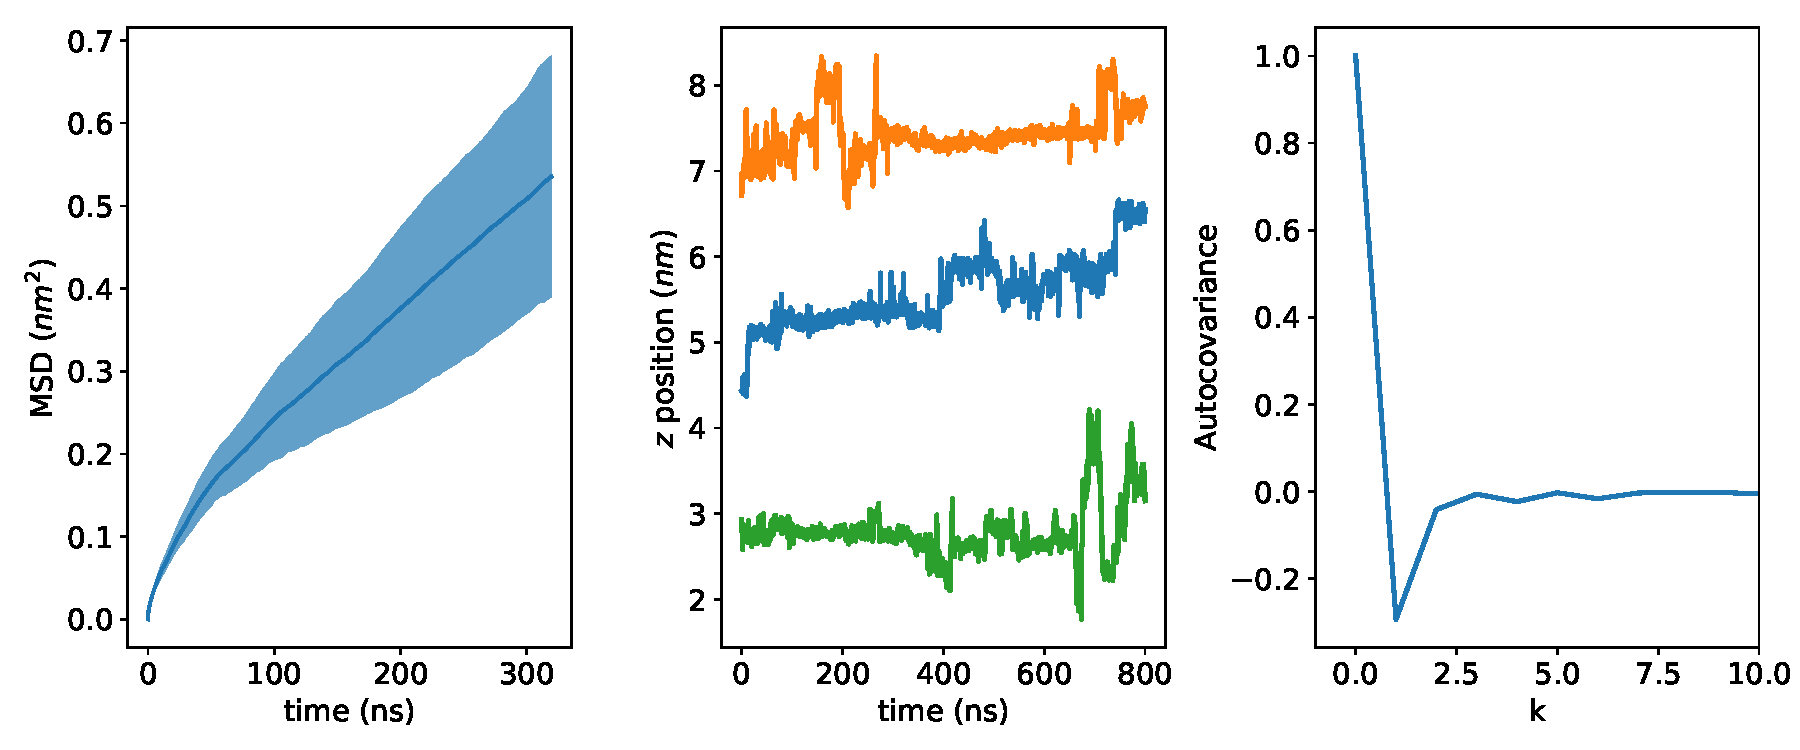
\includegraphics[width=\textwidth]{msd_ztrace_acf.pdf}
%  \caption{}\label{fig:msd_ztrace_acf}
%  \end{figure}

  \begin{figure}
  \centering
  \begin{subfigure}{0.49\textwidth}
  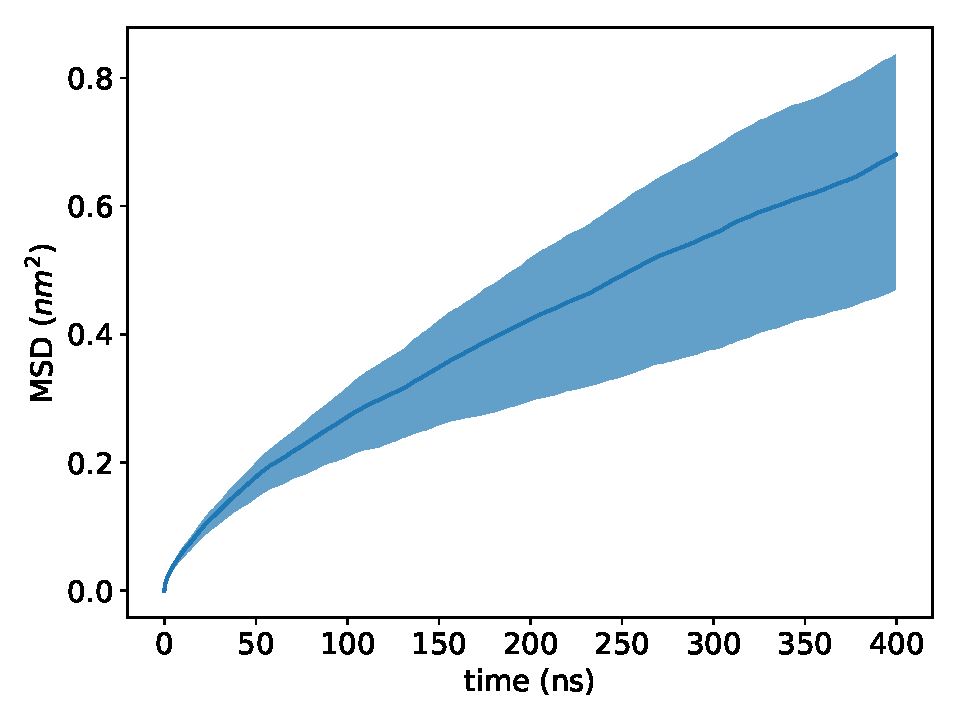
\includegraphics[width=\linewidth]{example_msd.pdf}
  \caption{}\label{fig:example_msd}
  \end{subfigure}
  \begin{subfigure}{0.49\textwidth}
  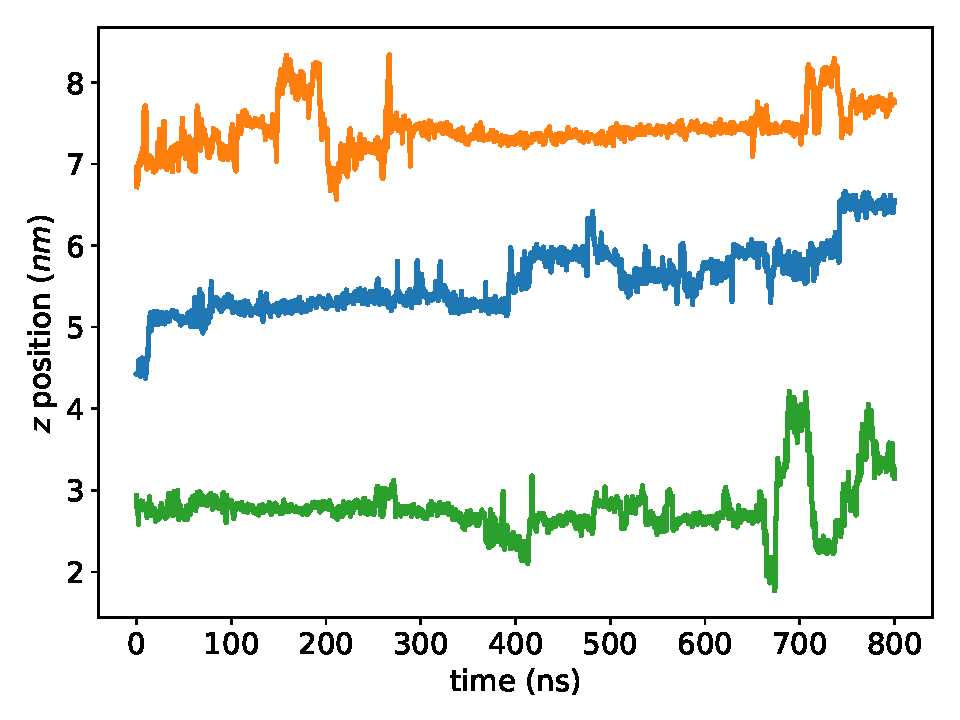
\includegraphics[width=\linewidth]{example_ztraces.pdf}
  \caption{}\label{fig:example_ztraces}
  \end{subfigure}
  \par\medskip
  \begin{subfigure}{0.325\textwidth}
  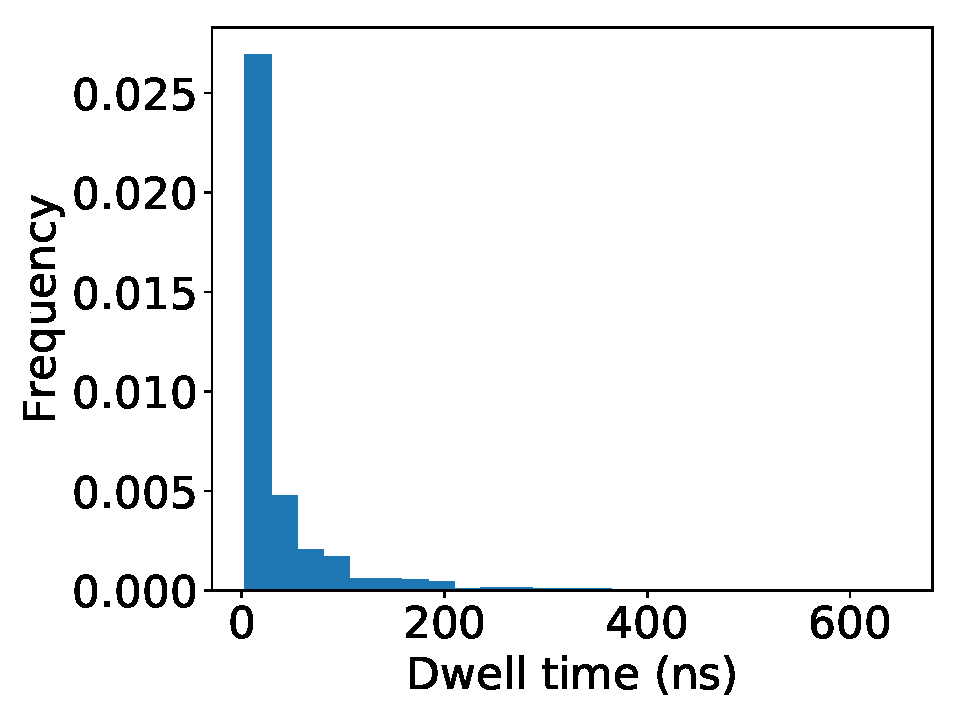
\includegraphics[width=\linewidth]{example_powerlaw.pdf}
  \caption{}\label{fig:example_powerlaw}
  \end{subfigure}
  \begin{subfigure}{0.325\textwidth}
  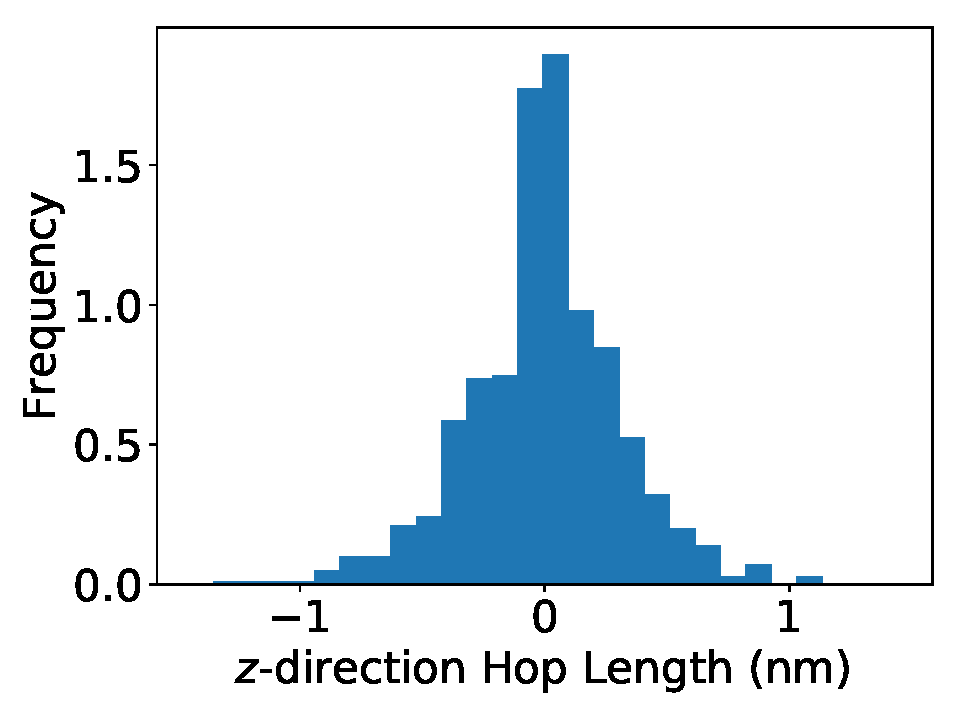
\includegraphics[width=\linewidth]{example_hop_dist.pdf}
  \caption{}\label{fig:example_hop_dist}
  \end{subfigure}
  \begin{subfigure}{0.325\textwidth}
  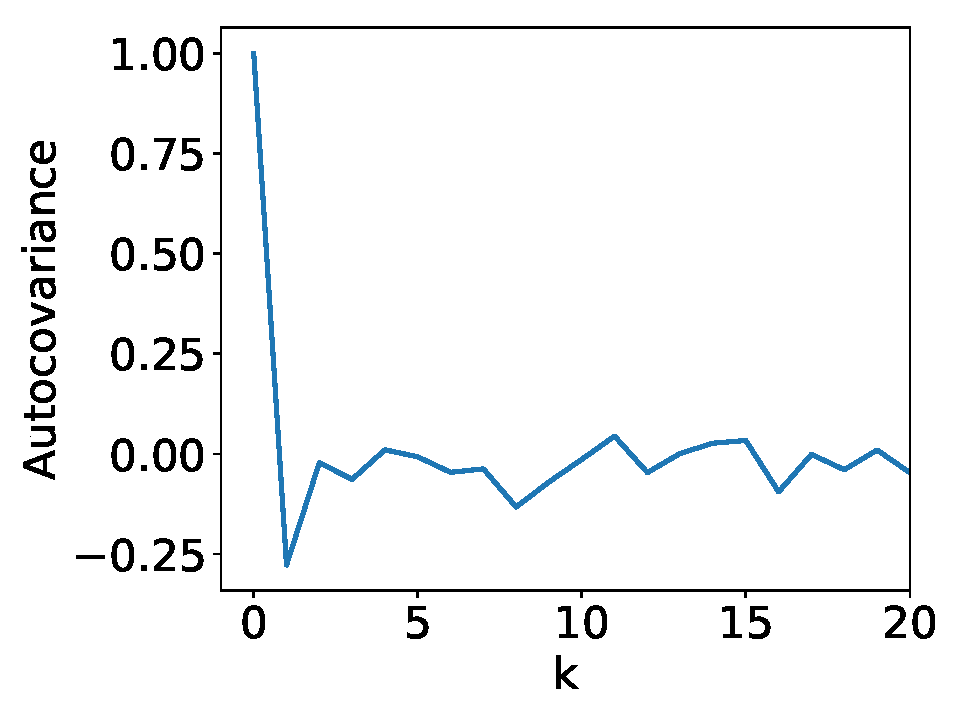
\includegraphics[width=\linewidth]{example_autocovariance.pdf}
  \caption{}\label{fig:example_autocovariance}
  \end{subfigure}
  \caption{All solutes show subdiffusive transport behavior inside the membrane's
  nanopores, similar to that exhibited by ethanol. (a) The time-averaged MSD of 
  ethanol is not linear which suggests transport is governed by an anomalous 
  subdiffusion process. (b) The $z$-coordinate trace of 3 representative ethanol
  COMs shows clear periods of entrapment separated by hops. (c) The distribution
  of dwell times follows a power law. (d) The distribution of hop lengths appears
  Gaussian. (e) Hops are anti-correlated to their previous hop as indicated by the
  negative value of the autocovariance function at $k$ = 1.}\label{fig:examples}
  \end{figure}
  
  % BJC: would it be better to report as a fraction of water MSD?
  % BJC: need MSDs of 5 wt % systems here too. Can narrow to study of 10 wt % systems after
  \noindent We calculated the time-averaged MSD of each solute in the set over the
  course of 1 $\mu$s MD simulations. 
  \begin{itemize}
    \item Because the MSDs are non-linear and because of the ageing phenomenon, we
    did not attempt to calculate a diffusion constant as one might for a Brownian
    particle with a linear MSD.
	\item Instead, the MSD values plotted in Figure~\ref{fig:all_msds} represent the
	average MSD of each solute after a 400 ns time lag.
  \end{itemize}  
  
%  \subsubsection*{The Influence of Water Content on Macroscopic Diffusion Coefficients}
%
%  Solutes in systems with lower water content exhibit lower diffusion coefficients.
%  \begin{itemize}
%	\item Pores are more crowded when there is less water (show RDFs of each)
%	\item Not a linear function of pore size - radius increase by x, D increases by y
%	\item Larger influence on bigger molecules
%  \end{itemize}
  
  \begin{figure}
  \centering
  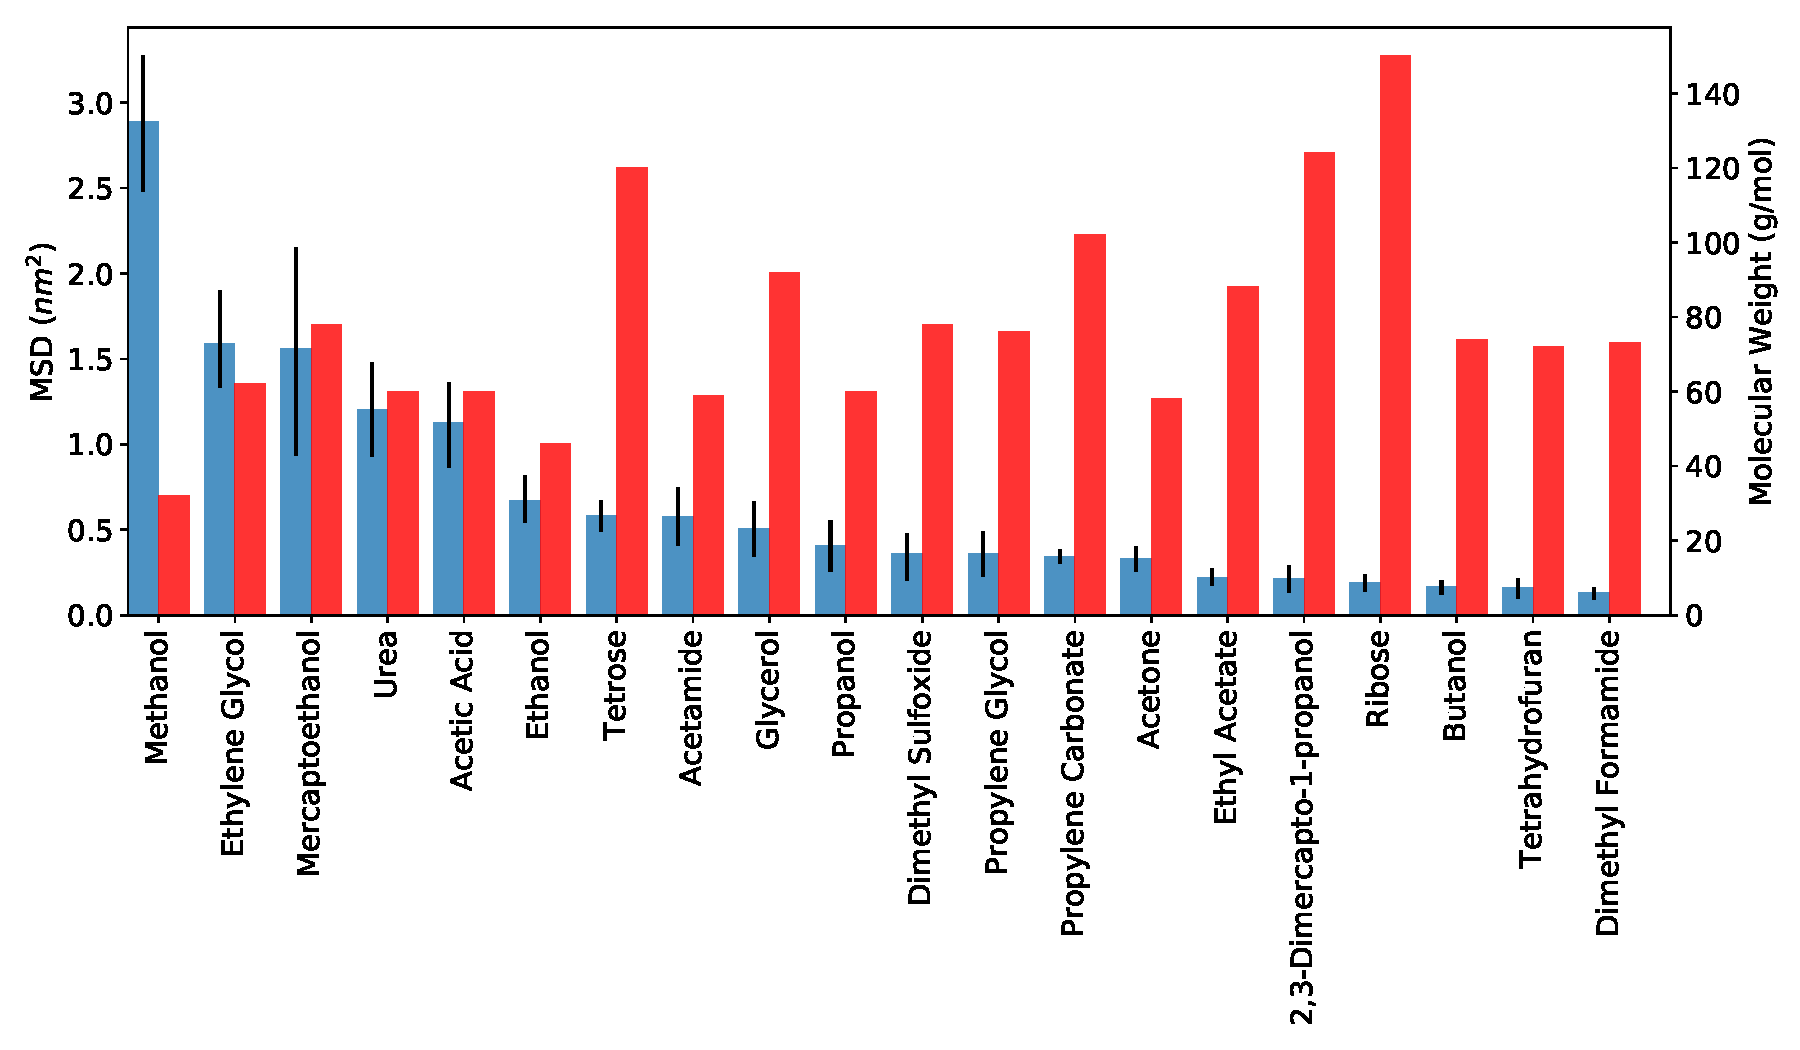
\includegraphics[width=\textwidth]{all_tamsds.pdf}  % include bar plot of MW to show it's non-monotonic
  \caption{}\label{fig:all_msds}
  \end{figure}
  
  \noindent The MSDs are not a monotonic function of solute molecular weight.
  \begin{itemize}
  	\item We plotted the solute molecular weights alongside their MSDs in Figure~\ref{fig:all_msds}.
  	\item Transport is clearly affected by factors other than molecular weight. 
  	\item Tetrose, our third heaviest solute, has an MSD higher than more than half of
  	all solutes studied. 
  	\item The three slowest solutes have lower molecular weights than 8 faster solutes.
  \end{itemize}
  
  \noindent The MSDs in Figure~\ref{fig:all_msds} are a strong function of two solute 
  trapping mechanisms. % by which solutes become trapped.
  \begin{itemize}
  	\item Solutes that are hydrogen bond donors can be stabilized through hydrogen bonds
  	with one of the five oxygen atoms attached to each monomer head group. 
  	\item In a separate interaction, solutes can become kinetically trapped between or behind
  	monomer head groups. These interactions likely lead to the observed anti-correlated
  	hopping	behavior.
  	\item Generally, both mechanisms affect each solute to varying degrees.
  \end{itemize}
  
  %BJC: somewhere need to say why solutes preferentially hbond with carboxylate groups -- is this real
  
  %BJC: This will need updating once all the rest of outline is written.
  \noindent The degree to which solutes are influenced by each entrapment mechanism
  is a complex function of a solute's size, shape, and polarity.
  \begin{itemize}
    \item In general, solutes can move fastest in the pore center, where
    there is comparatively little resistance to diffusion.
	\item The 5 fastest solutes in our study have a low molecular weight and
	spend a significant amount of time in the pore center. They are only slowed
	by hydrogen bonds with monomer carboxylate groups.
	\item Bulky solutes with many hydrogen bond donating groups, like glycerol,
	spend most of their time in the pore center, but their large size combined
	with a higher solute-head group hydrogen bond frequency, makes their dynamics slow. 
    \item Solutes with high hydrophobic character tend to partition into the 
    head group region where entrapment occurs.
    \item We observe low MW solutes with lower-than-expected MSDs because they
    spend more time trapped between monomer head groups due to low water
    solubility.
    \item Small, planar molecules, without the ability to donate hydrogen bonds, like acetone,
    exhibit some of the slowest MSDs. Their flat geometry and small size makes it easy for 
    them to get lodged deep between head groups.
  	\item Overall solutes exhibit some degree of trapping, by one or a combination of the above
  	mechanisms, with anticorrelated hops between each period of immobility due to 
  	obstructions.
  \end{itemize}
  
  %BJC: potential figure to go with above paragraph
  % (a) Plot showing how biggest jumps are at pore center
  % (b) Illustrate preference for hbonds carboxylate head groups
  
  We will revisit these observations in the the context of specific groups of 
  molecules in the discussion that follows.

%  We will explore these factors in greater detail in the context of 
%  specific groups of molecules in the discussion that follows.

  \subsection*{Transport of Water}

  The MSD of water is a weak function of the solute residue disolved in
  the pores.
  \begin{itemize}
  	\item Large molecules like glycerol and ribose obstruct the movement
  	of water molecules forcing them to have lower MSDs
  	\item I don't know why the MSD is fast in the fastest systems or why DMSO is slow.
  	\item Sulfur containing compounds have slowest water transport
  	\item How do 24 solute molecules have such a drastic effect on water motion
  \end{itemize}

  % BJC: MSDs only calculated for water molecules that spend > 95 % of their
  % time in the pore. Pore region / tail region cutoff is at 1.5 nm (approximate location of lowest radial water density) 
  \begin{figure}
  \centering
  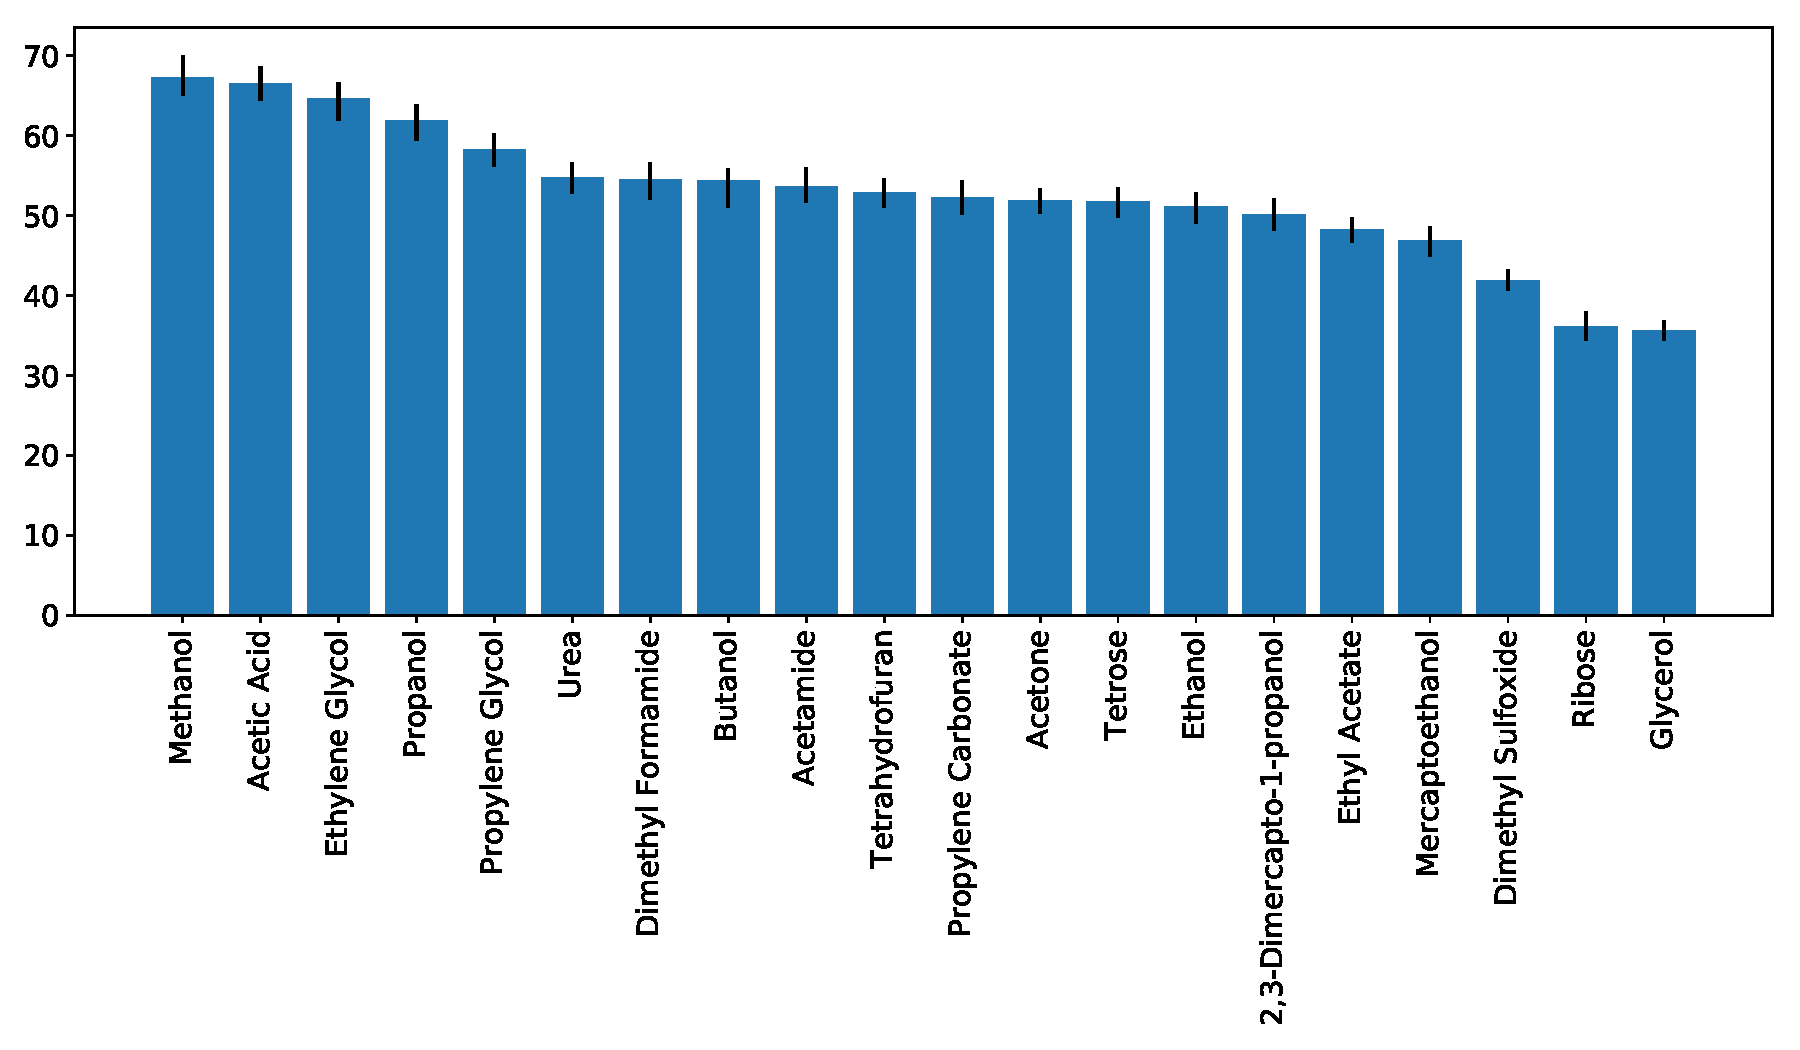
\includegraphics[width=\textwidth]{water_msd.pdf}
  \caption{}\label{fig:water_msd}
  \end{figure}
  
  % BJC. Other Notes:
  % There is no discernable trend in flux of water to/from pores. Most levels stay 
  % comparable to their initial values while a handful have ~50 water molecules that
  % enter the pore during the simulation.
  % Water molecules that spend > 95 % of their time within 1 nm of the pore center 
  % have lower MSDs -- although there aren't a lot of them to average over. They are
  % probably lower because they can't be moving much to stay so confined
  
  \subsection*{Transport of Simple Alcohols}

  The MSD of methanol, ethanol, propanol and butanol descends in order of 
  their molecular weight, however, methanol travels faster than expected.  %BJC: find approximate relationship between MW and mobility
  \begin{itemize}  
    \item The radial density as a function of distance from the pore center
    for each alcohol is plotted in Figure~\ref{fig:simple_alcohol_rdf}.
    \item On average, the density of methanol in the pore center is only slightly
    less than the density near the head groups.
    \item All other alcohol molecules are most concentrated in the head group region.
  \end{itemize}
  
  All simple alcohols participate in a similar number of hydrogen bonding interactions
  with the monomer head groups, but with varying preference towards hydrogen bonds with
  the monomer carboxylate oxygen atoms (See Figure~\ref{fig:simple_alcohol_hbonds}).
  \begin{itemize}
  	\item If all 5 hydrogen bonding acceptor sites on the monomer head groups were equal,
  	we would expect the ratio of the number of hydrogen bonds between solutes and the two 
  	carboxylate oxygen atoms to the number of hydrogen bonds between solutes and the three
  	ether groups to be 2/3. 
  	\item There is a clear preference towards hydrogen bonding with the carboxylate 
  	oxygen atoms for all simple alcohols.
  	\item This is largely due to the more highly crowded environment surrounding the ether
  	oxygen atoms.
  	\item Butanol shows the largest preference towards hydrogen bonds with carboxylate 
  	head groups.
  	\item The radial distribution function of atoms located at opposite ends of butanol
  	shows that, on average, oxygen atoms are situated 0.25 nm closer to the pore centers
  	than the distal carbon atoms.
  	\item This suggests that alcohols tend to orient themselves like the liquid crystal 
  	monomers, with hydrophilic components point towards the pore centers.
  \end{itemize}
  
  \begin{figure}
  \centering
  \begin{subfigure}{0.325\textwidth}
  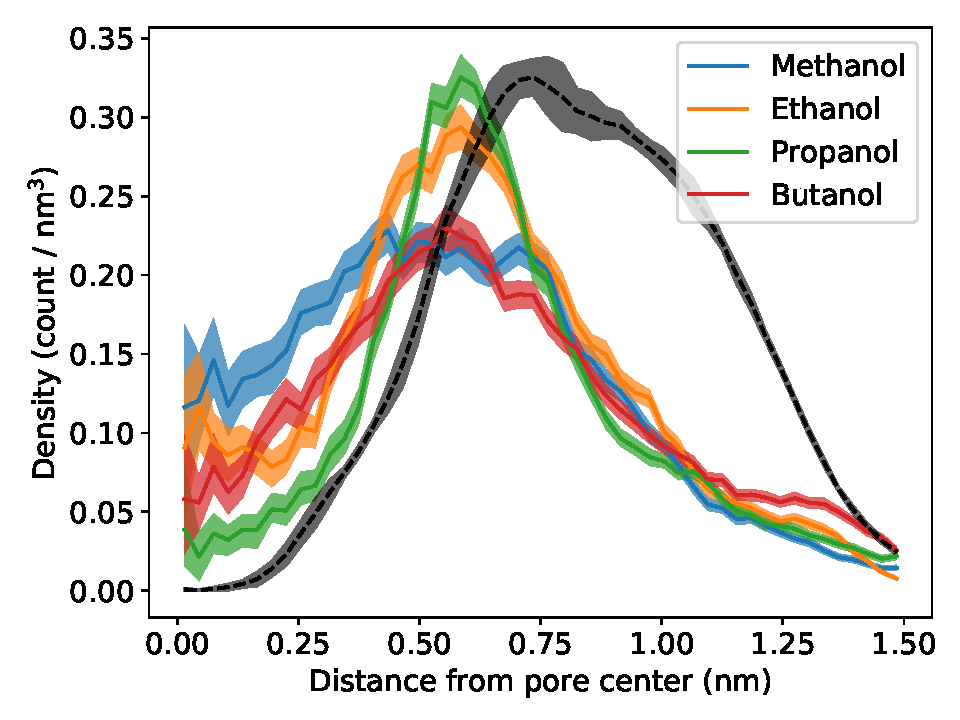
\includegraphics[width=\linewidth]{simple_alcohol_rdf.pdf}
  \caption{}\label{fig:simple_alcohol_rdf}
  \end{subfigure}
  \begin{subfigure}{0.325\textwidth}
  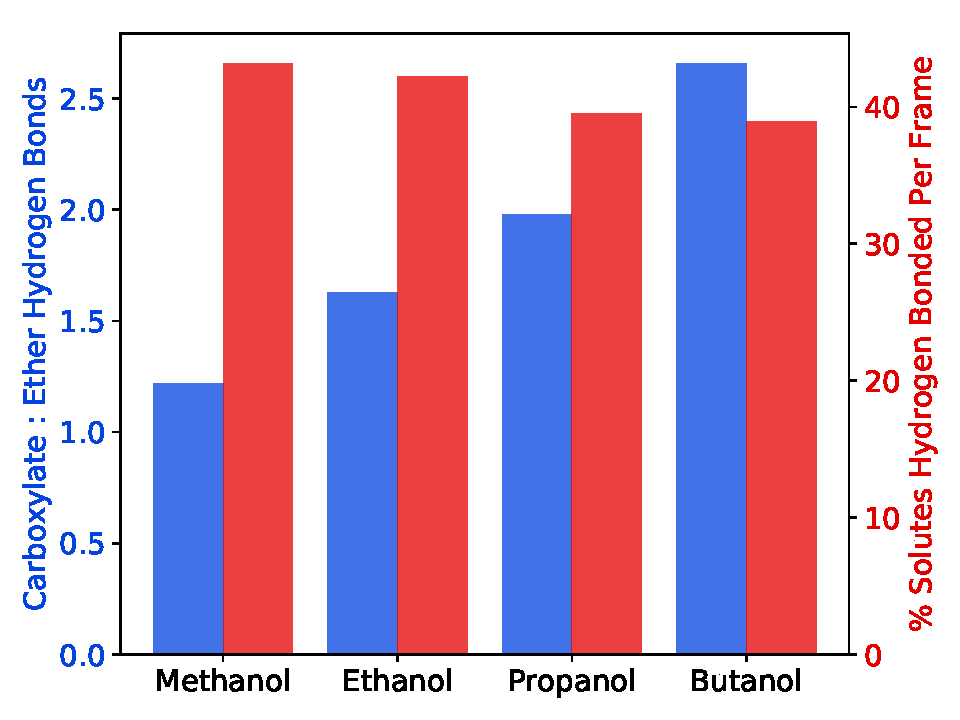
\includegraphics[width=\linewidth]{simple_alcohol_hbonds.pdf}
  \caption{}\label{fig:simple_alcohol_hbonds}
  \end{subfigure}
  \begin{subfigure}{0.325\textwidth}
  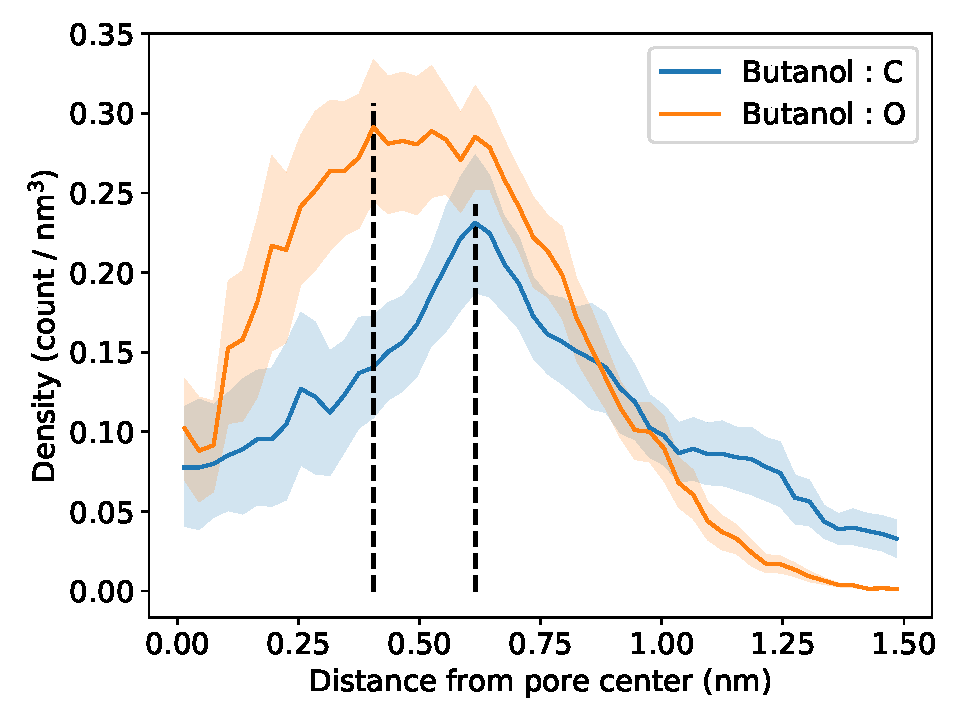
\includegraphics[width=\linewidth]{butanol_CO.pdf}  %BJC: can add inset to plot showing butanol with highlighted O and C
  \caption{}\label{fig:butanol_CO}
  \end{subfigure}
  \caption{(a) The radial distribution functions of each simple alcohol shows a maximum close
  to the highest density of monomer head groups (dashed line, normalized for easier visual
  comparison). Methanol spends the largest proportion of time, relative to the other alcohols,
  near the pore center, which may help explain its fast dynamics. (b) Despite relatively little
  difference in the total number of hydrogen bond occurences, a given alcohol's preference
  towards hydrogen bonds with the carboxylate groups increases with molecule size. (c) The average
  location of butanol's oxygen atom is significantly closer to the pore center than its most distal
  carbon atom, suggesting that the molecule is oriented with hydrophobic tails pointing away from
  the pore center.}\label{fig:simple_alcohols}
  \end{figure}

  \subsection*{Transport of Diols, Triols and Sugars}  % polyols instead of sugars?
  
  Transport is both facilitated and hindered by additional solute hydroxyl groups.
  \begin{itemize}
    \item Extra hydroxyl groups cause solutes to favor the water-rich pore region.
    where there is the least hindrance to movement.
    \item However, these extra hydroxyl groups facilitate a larger number of 
    hydrogen bond interactions that work to hold solutes in place (See Figure~\ref{fig:multi_hbonds}).
    \item At the same time, solute molecular weight increases, which inherently
    causes them to move more slowly.
    \item Ethylene glycol, the fastest solute in this grouping (and second fastest
    overall), obtains the best balance of both effects.
  \end{itemize}
  
  The number of hydrogen bonding interactions between solutes and head groups
  increases with the number of solute hydroxyl groups.
  \begin{itemize}
    \item These solutes frequently undergo simultaneous hydrogen bond interactions as
    shown in Figure~\ref{fig:multi_hbonds}. 
    \item For example, both hydroxyl groups of ethylene glycol can undergo hydrogen
    bonds with different hydrogen bond acceptors at the same time.
    \item In some cases, all 4 hydroxyl groups of ribose are hydrogen bonded to monomer
    head groups simultaneously.
  \end{itemize}
  
  \begin{figure}[!htb]
  \centering
  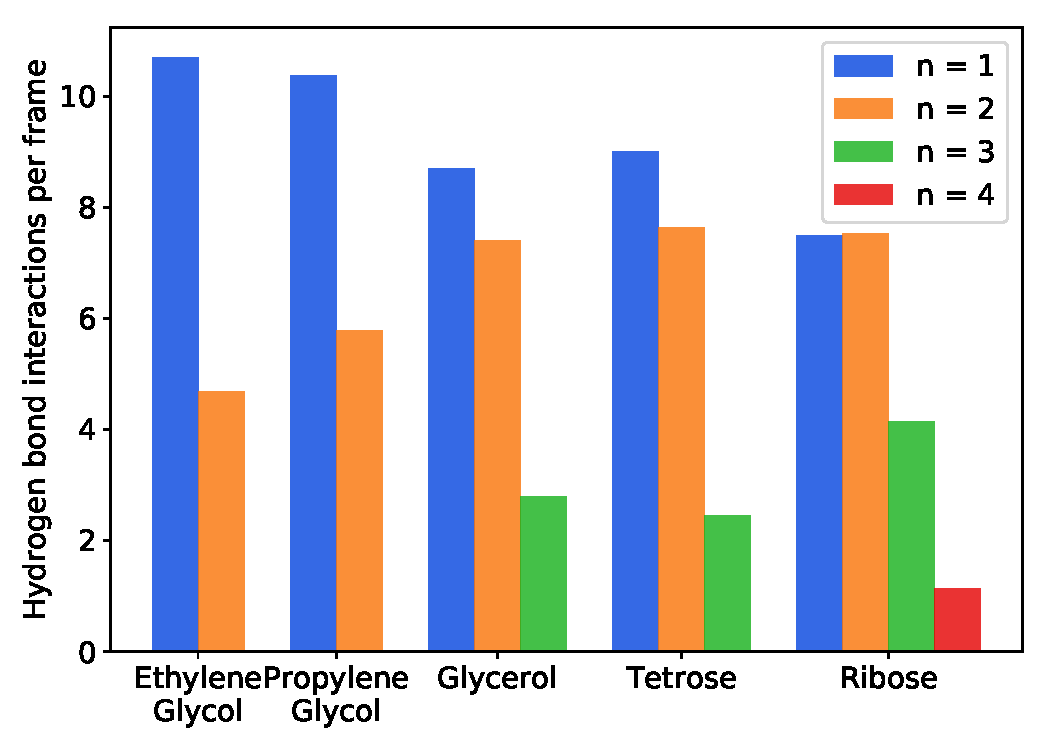
\includegraphics[width=\linewidth]{multi_hbonds.pdf}
  \caption{The number of hydrogen bond interactions between solutes and monomers increases
  as solutes gain additional hydroxyl groups. Multiple hydroxyl groups within a solute often
  hydrogen bond in different locations simultaneously. Occasionally, all four hydroxyl groups
  of Ribose (n = 4) are involved in a hydrogen bond interaction at the same time.}\label{fig:multi_hbonds}
  \end{figure}
  
  Between the two diols, ethylene glycol moves significantly faster than propylene glycol
  due to propylene glycol's affinty for the monomer head groups.  
  \begin{itemize}
  	\item The distribution of each solute's dwell time and hop length distributions shows that
  	ethylene glycol has shorter dwell times and longer hop lengths, which combine to create a 
  	relatively fast MSD. 
  	%BJC: number of PG vs ethylene glycol that enters middle -- I don't think this will be any different than density function
    \item Both diols have comparable densities close to the pore center, however propylene glycol's
    density has a large peak near the monomer head groups relative to ethylene glycol. 
    \item Combined with an increase in molecular weight, the addition of a single methyl group
    increases the molecule's hydrophobic character and causes propylene glycol to favor positions
    near monomer head groups.
    \item This causes propylene glycol to form more highly stablized hydrogen bonds with
    carboxylate groups, explaining the higher incidence of hydrogen bonds shown in Figure~\ref{fig:multi_hbonds}.
  \end{itemize}
  
  % BJC: figure does not represent total number of hops (PG has less hops)
  \begin{figure}[!htb]
  \centering
  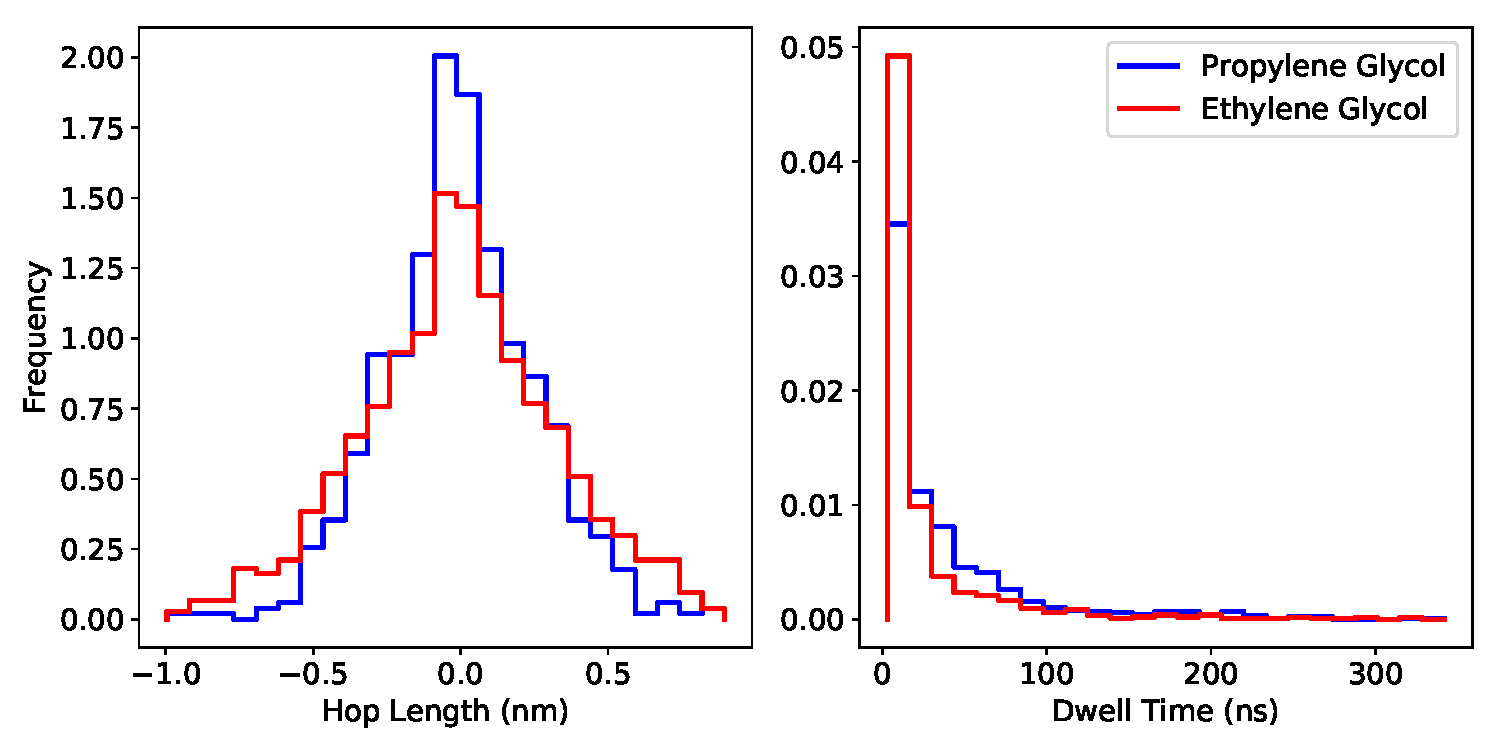
\includegraphics[width=\linewidth]{dwell_hop_PG_GCL.pdf}
  \caption{}\label{fig:dwell_hop_PG_GCL}
  \end{figure}
  
  Solutes with three or more hydroxyl groups have the highest density
  at the pore center which contributes to overall faster than expected transport.
  \begin{itemize}
  	\item These molecules are highly water soluble but relatively large
  	\item They can easily hydrogen bond in multiple locations.
  	\item Their large size and high hydrogen bonding capability prevents them
  	from having larger MSDs.
  \end{itemize}
  
  % BJC: Euclidean distance between simultaneous h-bonds for ethylene glycol?
  
%  Ethylene glycol, a diol, has two hydrogen bond donor groups.
%  \begin{itemize}
%	\item Can hydrogen bond with same moeity.
%	\item Can hydrogen bond with different moeities in the same 
%	vicinity. 
%	\item Dwell times tend to be shorter. If one hydroxyl group is bound
%	with a hydrogen bond, the other unbound hydroxyl group may form a hydrogen bond
%	elsewhere and effectively pull the other bound hydroxyl group along with it. 
%  \end{itemize}

  \subsection*{Transport of Ketones and Amides}
  
  The 4 ketone-like molecules tested show a surprising range of transport behaviors.
  \begin{itemize}
    \item Urea, Acetic Acid, Acetamide and Acetone are all characterized by a carbonyl group
    with two attached heavy atoms. 
    \item All have approximately the same molecular weight and are planar molecules due to
    the sp2 hybridization of the carbonyl group.
    \item The fastest solute of this grouping, Urea (comparable to Acetic Acid too), has an
    MSD comparable to that of ethylene glycol while the slowest, Acetone, has an MSD one 
    third of that of Urea.
  \end{itemize}
  
  Once again, the trends in the MSD can in large part be explained by the solutes'
  preference for water.
  \begin{itemize}
  	\item Urea, Acetic Acid and Acetamide are all capable of donating hydrogen bonds,
  	while acetone is the first instance of a molecule in this study that can only
  	accept hydrogen bonds. It follows that acetone has the slowest MSD of this grouping.
  	\item Urea and Acetamide both have hydrogen bond donating nitrogen atoms, however
  	nitrogen is a weaker hydrogen bond donor than oxygen due to its lower electronegativity.
  	\item Hence, Acetic Acid donates the greatest number of hydrogen bonds and has
  	the highest density throughout the pore region.
  	\item All other solutes show a higher preference for the tail region where three 
  	dimensional confinement directly contributes to a lower MSD.
  	\item Urea likely compensates for its loss of mobility in the head group region by
  	making large hops upon escape into the pore region.
  	\item Urea frequently moves between the head group and pore region because its planar
  	shape makes it easier to transition between regions.% could quantify transition frequency probably. It seems like it might yield something. But also might make things more ambiguous.
  	\item As the solutes become less polar, their MSD decreases. 
  	\item Acetamide has one less amine group than Urea and a corresponding smaller MSD.
  	\item Despite a peak in its density near the pore center due to its water solubility,
  	Acetone is the least polar and spends the most time outside the tail group region 
  	leading to the lowest MSD.
%  	\item With two nitrogen groups that hydrogen bond relatively infrequently, one might 
%  	expect Urea to exhibit much faster transport, however its MSD is comparable to
%  	the much stickier acetic acid. 
%  	\item Urea is highly soluble in water but not miscible in all proportions like 
%  	acetic acid or even acetone.
%  	\item Relative to acetic acid, acetamide, urea and acetone spend more time in the head group region.
%  	\item There is a large peak near the head groups, but \% of the urea molecules 
%  	are behind in the head group region.
%  	\item The structure of acetamide differs from acetic acid only by an amine group in place
%  	of a hydroxyl group.
%  	\item The weaker hydrogen bonding capability of acetamide and an extra nonpolar methyl group compared to
%  	Urea makes acetamide even more likely to partition. 
%  	\item Urea has two hydrogen bond donor nitrogen atoms. It is not surprising that
%  	its density is high near the pore center, particularly near the monomer head groups.
%  	
%  	\item Acetic acid, a carboxylic acid shows a relatively high density in the pore region, with 
%  	a peak close to the carboxylate groups.  %BJC: hbonds a lot 
%  	\item Acetone is stabilized by accepting hydrogen bonds from water in the pore region, but
%    its low polarity and planar shape gives it comparable stability when trapped between head groups.
%  	\item Acetone's has two prominent peaks in its radial density. One is in the pore region and the o
%  	other is relatively deep in the head group region.
  \end{itemize}
  
  \begin{figure}[!htb]
  \centering
  \begin{subfigure}{0.45\textwidth}
  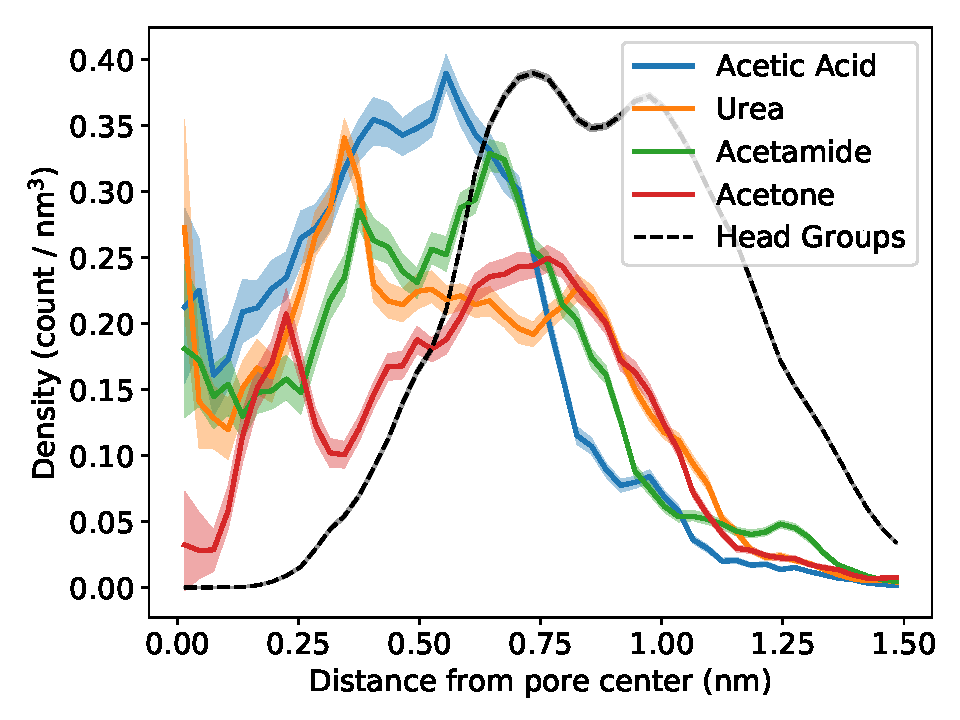
\includegraphics[width=\textwidth]{ketone_rdf.pdf}
  \caption{}\label{fig:ketones_rdf}
  \end{subfigure}
  \begin{subfigure}{0.45\textwidth}
  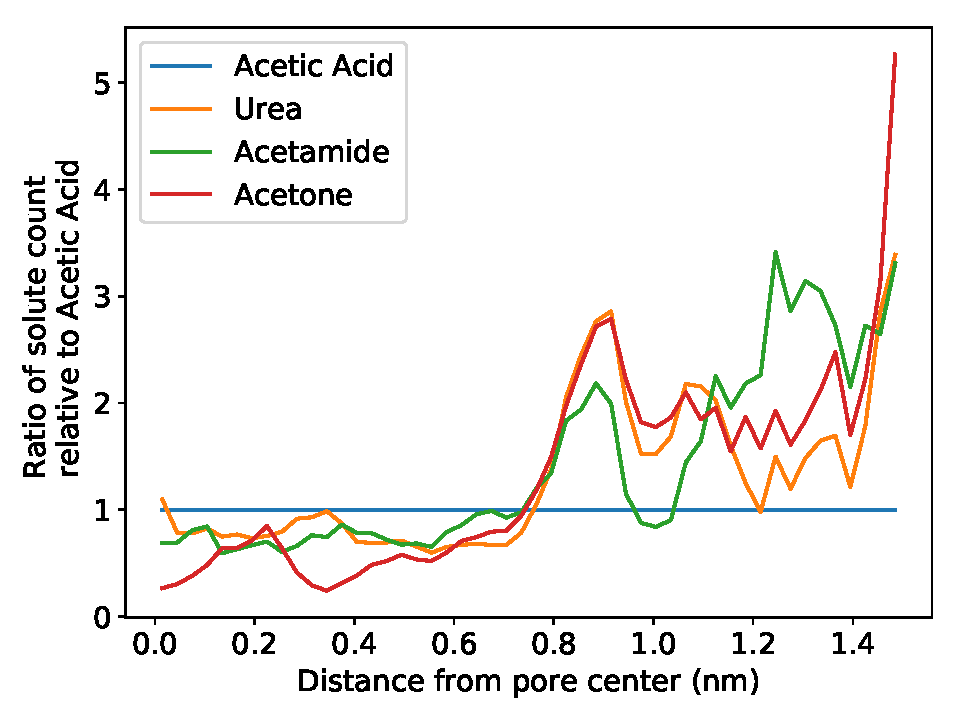
\includegraphics[width=\textwidth]{ketone_ratio.pdf}
  \caption{}\label{fig:ketones_ratio}
  \end{subfigure}
  \end{figure}
  
  \subsection*{Transport of Thiols}
  
  We also studied the transport properties of sulfur analogs of glycerol, ethylene
  glycol and acetone.
%  Finally, we studied the transport properties of sulfur-containing compounds similar
%  to some of the solutes studied above.
  \begin{itemize}
    \item We replaced all but one oxygen atom of ethylene glycol and glycerol with sulfur atoms
    to create Dimercaptoethanol and 2,3-Dimercapto-1-propanol.
    \item We replaced the carbonyl carbon of acetone with sulfur in order to create DMSO. 
  	\item Sulfur is unable to hydrogen bond, however it is soluble in water  %BJC: maybe a reference to why sulfur can't hbond
  	\item Comparisons of their RDFs are shown in Figure~\ref{fig:sulfur_analog_rdfs}.
  \end{itemize}
  
  \begin{figure}
  \centering
  \begin{subfigure}{0.325\linewidth}
  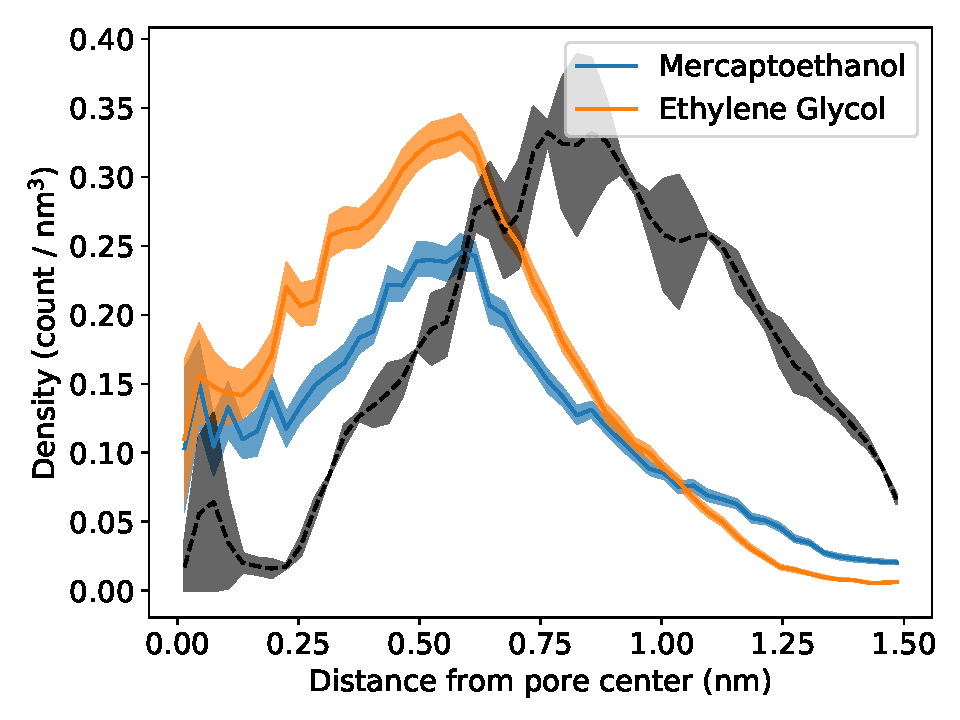
\includegraphics[width=\textwidth]{thiol_comparison_SOH.pdf}
  \caption{}\label{fig:SOH_GCL_comparison}
  \end{subfigure}
  \begin{subfigure}{0.325\linewidth}
  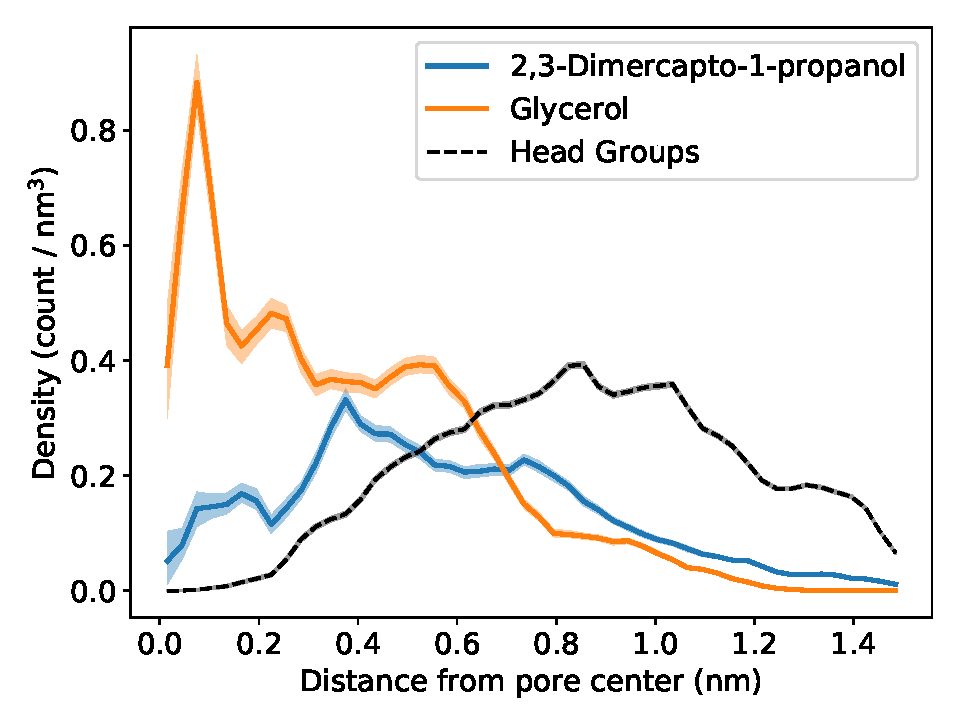
\includegraphics[width=\textwidth]{thiol_comparison_DMP.pdf}
  \caption{}\label{fig:DMP_GLY_comparison}
  \end{subfigure}
  \begin{subfigure}{0.325\linewidth}
  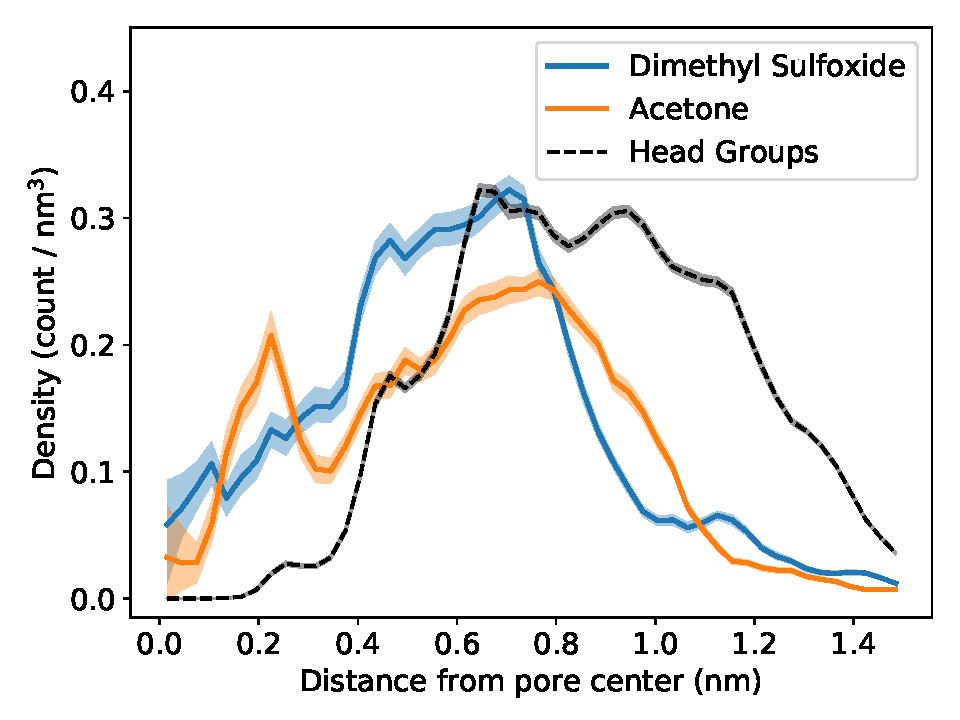
\includegraphics[width=\textwidth]{thiol_comparison_DMS.pdf}
  \caption{}\label{fig:DMP_GLY_comparison}
  \end{subfigure}
  \caption{}\label{fig:sulfur_analog_rdfs}
  \end{figure}
  
  \noindent Mercaptoethanol has a similar average RDF and MSD to ethylene glycol.
  \begin{itemize}
    \item There is a much larger uncertainty associated with mercaptoethanol's MSD.
    \item It spends more time in the tail region than ethylene glycol, where transport
    is inherently slower, and may contribute to some slower MSDs.  % Can quantify as a percentage
    \item Conversely, Mercaptoethanol also exhibits some of the highest single solute MSDs  % Only methanol has greater (I think)
    \item It hydrogen bonds with head groups 6 times less frequently than ethylene glycol.
    \item This may lead to larger hops in the pore region.
    \item Some of this can be accounted for by the higher density of mercaptoethanol 
    molecules in the head group / tail region. There are nearly 40 \% more mercaptoethanol
    molecules than ethylene glycol molecules beyond 0.8 nm from the pore center. 
%    \item When both hydroxyl groups of ethylene glycol are hydrogen bonded with the a
%    monomer head group simultaneously,
%    \item Less frequent hydrogen bonding and an affinity for the pore region may be
%    responsible for these hops.
  \end{itemize}
  
  \begin{figure}
  \centering
  \begin{subfigure}{0.45\textwidth}
  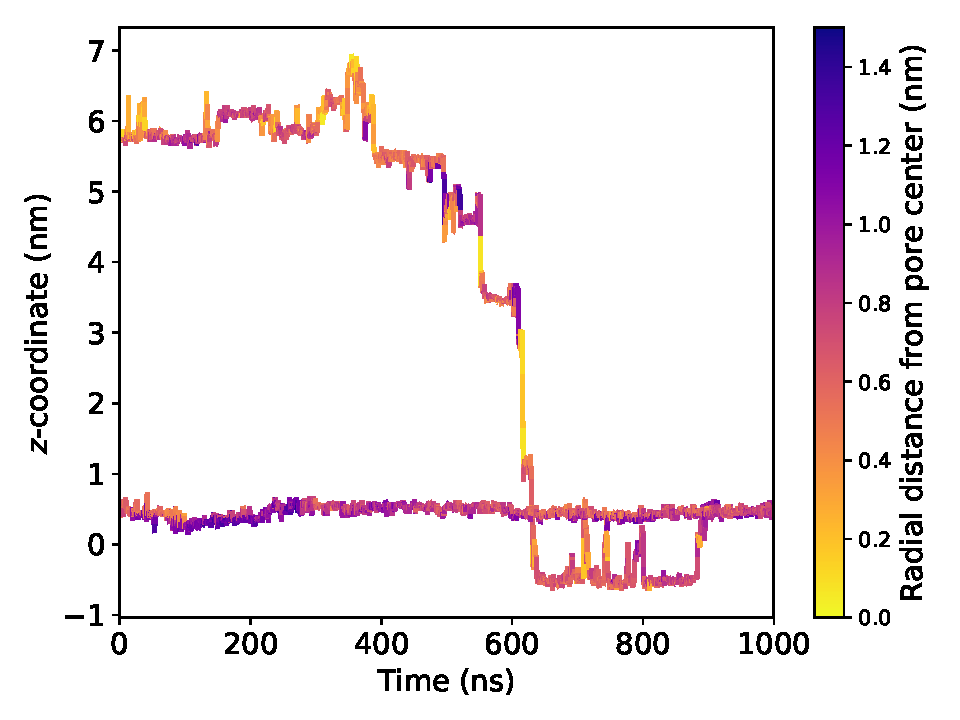
\includegraphics[width=\linewidth]{SOH_trace.pdf}
  \caption{}\label{fig:SOH_trace}
  \end{subfigure}
  \caption{}
  \end{figure}
  
  % Potentially useful explanation
%  Ethylene glycol has a high chance of hydrogen bonding at least once with monomer head groups. 
%  An ethylene glycol molecule can hydrogen bond twice simultaneously.
%  When one of those hydrogen bond breaks, the molecule is still stabilized by another hydrogen bond
%  It can easily reform the second hydrogen bond in close proximity
  
  \noindent 2,3-Dimercapto-1-propanol exhibits slower transport than glycerol because it spends more time
  near monomer head groups. % BJC: should I give all the solutes nicknames (i.e. their residue names)?
  \begin{itemize}
    \item Glycerol frequently hydrogen bonds with more than one head group at a time.
    % BJC: can probably quantify the following:
    \item It also hydrogen bonds with water molecules which increases its stability
    in the pore region.
    \item 2-3-Dimercapto-1-propanol preferentially hydrogen bonds with head groups 
    so it gravitates towards the head group region.
  \end{itemize} 
  
  \noindent DMSO has a comparable MSD to acetone even though its molecular weight is
  about 25 \% larger.
  \begin{itemize}
  	\item The pyramidal structure of DMSO may force it to spend more time closer to
  	the pore center.  % BJC: might be a good place for a numbers comparison
  	\item There are 20 \% more acetone than DMSO molecules in the region beyond 
  	0.8 nm from the pore center.  % based on actual number, not density
  	\item DMSO cannot as easily work its way in and out of the dense head group region. % BJC: some kind of average regional lifetime
  	\item There is a peak in DMSO's radial density near 1.1 nm which may be a consequence of 
  	solute molecules that get stuck in the tails.
  \end{itemize}  
  
  \subsection*{Hydrogen bond acceptors}  % Need a better heading since all molecules in this study are acceptors
  
  The final set of molecules we studied can accept hydrogen bonds, but cannot donate
  them. 
  \begin{itemize}
  	\item Among this set are the two slowest solutes in our study: Tetrahydrofuran and Dimethyl Formamide.
  	\item Ethyl acetate and Propylene Carbonate are only marginally faster, however they
  	are both larger molecules. %BJC: not sure how far I should dive into this point
  \end{itemize}
  
  The radial density functions highlight the solutes' preference for the 
  head group region.
  \begin{itemize}
  	\item There are small peaks in the radial density greater than 1 nm 
  	from the pore center.
  	\item The solutes become trapped in these regions where each step is
  	highly anti-correlated to its previous step, leading to very low MSDs.
  	\item The large size and nonplanar shapes of ethyl acetate and propylene 
  	carbonate may destabilize entrapment in the tail region more quickly, leading
  	to slightly faster transport. 
  	% BJC:  Ethyl acetate spends all of its time in a linear or near-linear conformation.
%  	\item The relatively small amount of movement on the timescales studied 
%  	do not reveal definitive reasons
  	\item Overall, 
  \end{itemize}
 
  \begin{figure}
  \centering
  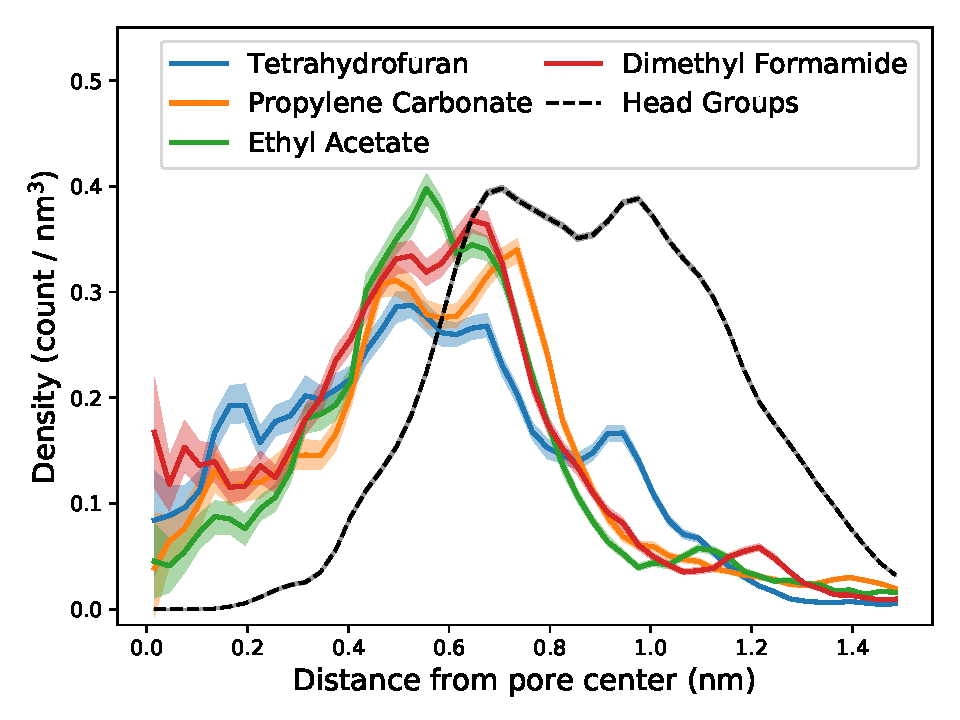
\includegraphics[width=0.45\textwidth]{nondonors_rdf.pdf}
  \caption{}\label{fig:nondonors_rdf}
  \end{figure}
  
  % THF shows highly anticorrelated hops
  
  %All have comparable densities near pore center except acetone which is lower

  \subsection*{Transport of Ions} % probably just sodium

  Sodium ions coordinate with water molecules.

%  Sodium ions also exhibit hop diffusion because polarized water and
%  carboxylate head groups both work to neutralize its charge.
%  \begin{itemize}
%	\item Ions get trapped in oxygen 'cages' composed of combinations
%	of water molecules, carboxylate head groups and ether oxygens connecting
%	the head groups to their tails.
%  	\item Interesting coordination number data
%	\item Dwell time proportional to surrounding charge within coordination shell
%  \end{itemize}

  \subsection{Design Principles}

  Water content affects pore size and strongly influence the MSD of both solutes and
  water. Experiments to understand how controllable this parameter is could be useful.
  
  Monomers that cannot hydrogen bond. % Hard to make a monomer like this

  Separate polar molecules by creating monomers with head group components designed to
  hydrogen bond.
  \begin{itemize}
  	\item Hbond donors
	\item More incentive to dwell on walls.
  \end{itemize}

  \section{Conclusion}

  We have examined the transport characteristics of a series of small polar
  molecules in our model of the H\textsubscript{II} phase formed by 
  Na-GA3C11.

  We calculated the macroscopic diffusion coefficients of each solute as 
  approximated by a CTRW model and validated our estimates using experimental
  DOSY NMR measurements.

  We have studied the influence of water content on the diffusion coefficients.

  We showed that hydrogen bonding between solutes and Na-GA3C11 monomers plays
  a major role in mechanism by which molecules traverse the nanopores. 

  We can use this intuition in order to modify our monomers for a specific 
  separation.
  \begin{itemize}
	\item Increase number of h-bond sites to increase selectivity towards water 
	over polar molecules
  \end{itemize}
  
 
  \section*{Supporting Information}

  Detailed explanations and expansions upon the results and procedures mentioned in
  the main text are described in the Supporting Information. This information is
  available free of charge via the Internet at http://pubs.acs.org.

  \section*{Acknowledgements}

  Molecular simulations were performed using the Extreme Science and
  Engineering Discovery Environment (XSEDE), which is supported by National
  Science Foundation grant number ACI-1548562. Specifically, it used the Bridges
  system, which is supported by NSF award number ACI-1445606, at the Pittsburgh
  Supercomputing Center (PSC). This work also utilized the RMACC Summit supercomputer,
  which is supported by the National Science Foundation (awards ACI-1532235 and
  ACI-1532236), the University of Colorado Boulder, and Colorado State
  University. The Summit supercomputer is a joint effort of the University of
  Colorado Boulder and Colorado State University.

  \clearpage

  \bibliographystyle{ieeetr}
  \bibliography{transport}

  \newpage

  \section*{TOC Graphic}

\end{document}
